\documentclass[a4paper,12pt]{article}
\usepackage[a4paper,top=1.3cm,bottom=2cm,left=1.5cm,right=1.5cm,marginparwidth=0.75cm]{geometry}
%%% Работа с русским языком
\usepackage{cmap}					% поиск в PDF
\usepackage{mathtext} 				% русские буквы в фомулах
\usepackage[T2A]{fontenc}			% кодировка
\usepackage[utf8]{inputenc}			% кодировка исходного текста
\usepackage[english,russian]{babel}	% локализация и переносы

\usepackage{graphicx}
\usepackage{mathtools}
\usepackage{wrapfig}
\usepackage{tabularx}
\usepackage{amssymb}
\usepackage{hyperref}
\usepackage[rgb]{xcolor}
\hypersetup{colorlinks=true,urlcolor=blue}
\setcounter{secnumdepth}{0}
%% Шрифты
\usepackage{euscript}	 % Шрифт Евклид
\usepackage{amsmath}
\usepackage{mathtools}
%%% Заголовок
\author{Tsvetkova Amelia}
\title{Лабораторная работа по общей физике}

\date{\today}
\begin{document}
\begin{titlepage}
    \newpage
    \begin{center}
    {\large МОСКОВСКИЙ ФИЗИКО-ТЕХНИЧЕСКИЙ ИНСТИТУТ (НАЦИОНАЛЬНЫЙ ИССЛЕДОВАТЕЛЬСКИЙ УНИВЕРСИТЕТ)}
    \vspace{1cm}

    {\largeФизтех-школа аэрокосмических технологий}
    \vspace{6em}
    \end{center}
    
    \vspace{1.2em}

    \begin{center}
    \Large Лабораторная работа №4.6.2 \\
    Туннелирование миллиметровых радиоволн
    \linebreak
    \end{center}
    
    \vspace{11em}
    
    \begin{flushright}
                       {\large Работу выполнила\\
                       Цветкова Амелия Антоновна\\
                       Б03-303 }
    \end{flushright}

    \vspace{\fill}

    \begin{center}
    Долгопрудный, 2025
    \end{center}

    \end{titlepage}

\paragraph{Цель работы:} экспериментальное исследование эффекта проникновения электромагнитных волн - туннелирования - через воздушный зазор между диэлектрическими призмами при полном внутреннем отражении на границе диэлектрик-воздух, а также моделирование интерферометра Майкельсона с использованием этого эффекта и измерение длины волны излучения и показателя преломления фторопласта для радиоволн миллиметрового диапазона.

\paragraph{В работе используются:} генератора СВЧ-колебаний с рупорной антенной; приемная рупорная антенна и волновод; детектор; микроамперметр; металлические зеркала; две призмы и плоскопараллельная пластина из фторопласта; микрометрические винты.

\section{Теоретические сведения}
\subsection{Генерация СВЧ-радиоволн}

Полоса сверхвысоких частот(СВЧ) $3 \text{ГГц} \leq \nu < 30 \text{ГГц}$ отвечает сантиметровому диапазону ($1 \text{см} < \lambda \leq 10 \text{см}$). В качестве источников ЭМ-излучения малой мощности обычно используются генераторы на $\textit{отражательных клистронах}$. Отражательный клистрон, изображенный на рис.$\ref{img1}$, представляет собой электровакуумный прибор, имеющий один тороидальный резонатор 1, дважды пронизываемый электронным потоком 2. Возвращение электронов осуществляется с помощтью отражателя 3, находящегося под отрицательным постоянным потенциалом $U_{\text{отр}}$ по отношению к катоду.

\begin{figure}[h]
\centering
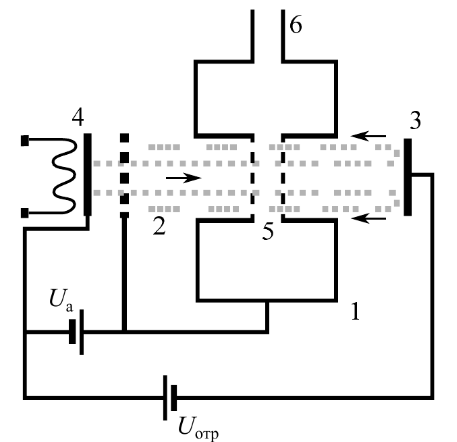
\includegraphics[width=0.4\linewidth]{img1.png}
\caption{Схема отражательного клистрона}
\label{img1}
\end{figure}

Процесс генерации протекает следующим образом. Электроны, эмитируемые катодом 4, ускоряются постоянным анодным напряжением $U_a$ и попадают в узкий сеточный зазор резонатора 5, в котором имеется продольное высокочастотное электрическое поле. Это поле периодически ускоряет и замедляет электроны, модулируя электронный поток по скорости. Двигаясь далее, электроны образуют сгустки за счет того, что быстрые электорын догоняют медленные. При обратном пролете они проходят через резонатор, когда в нем имеется тормозящее высокочастотное поле. Часть кинетичсекой энергии преобразуется в энергию резонатора, компенсируя затраты на полезное излучение.

Энергия СВЧ-колебаний из клистрона поступает в \textit{радиоволновод} 6, по которому распространяется в виде бегущей ЭМ-волны к нагрузке, в роли которой при излучении в открытое пространство выступает антенна. Особенно эффективна антенна в форме рупора, который улучшает согласование с открытым пространством, из-за чего увеличивается излучаемая мощность. Чем шире раскрыв рупорной антенны, тем уже направленным будет излучение.

\subsection{Распространение ЭМ-волн в радиоволноводах}

Радиоволноводы служат для транспортировки электромагнитной энергии в интервале длин волн от 1 м до 1 мм. Волноводы делаются из металлических труб и могут иметь любой профиль (делаются круглые или прямоугольные). В миллиметровом диапазоне волноводы могут быть сделаны из диэлектрика. 

Построим ЭМ-поле в волноводе, с помощью метода Бриллюэна, складывая падающую и отраженные от стенок плоские волны.

Плоские электромагнитные волны, рапспространяющиеся в однородной изотропной среде:
$$
\vec{E}(\vec{r}, t) = \vec{E_0} e^{i(\vec{k}\vec{r}-wt)} = \vec{A}(\vec{r})e^{-iwt}
$$
Здесь $\vec{E_0}$ - амплитуда напряженности электрического поля $\vec{E}$, $\vec{r}(x,y,z)$ - радиус-вектор точки наблюдения, $t$ - время, $w = 2\pi\nu$ - круговая частота, $\vec{k}(k_x,k_y,k_z)$ - волновой вектор. Направление вектора $\vec{k}$ совпадает с направлением распространения волны, а его модуль равен 
$$k = \frac{2\pi}{\lambda}=\frac{w}{v}$$
где $v$ - фазовая скорость волны, которая в пустом пространстве совпадает со скоростью света $c$. Векторная величина
$$\vec{A}(\vec{r})=\vec{E_0} e^{i\vec{k}\vec{r}} = \vec{E_0}e^{i(k_xx+k_yy+k_zz)}$$
называется комплексной амплитудой волны.

Рассмотрим отражение плоской ЭМ-волны от идеально проводящей, бесконечно протяженной плоской поверхности $x = 0$ (рис.$\ref{img2}$). Оба вектора поля $\vec{E}$ и $\vec{H}$ лежат в плоскости одинаковой фазы волны, им перпендикулярен волновой вектор $\vec{k}$, составляющий с векторами поля правую тройку.

\begin{figure}[h]
\centering
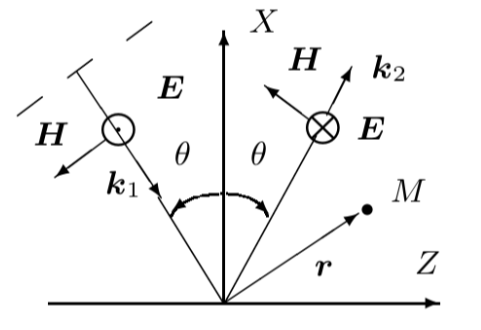
\includegraphics[width=0.3\linewidth]{img2.png}
\caption{Отражение плоской волы от проводящей поверхности}
\label{img2}
\end{figure}

В произвольную точку M над проводящей плоскостью приходятся падающая волна с напряженностью $\vec{E_\text{пад}}$ и отраженная от плоскости с $\vec{E_\text{отр}}$. Из граничного условия: $\vec{E_\tau}(t) = 0$, вытекает, что в отраженной и падающей волнах совпадают углы падения и отражения, частоты, волновые числа и модули амплитуд.
$$
\vec{E_\text{пад}} = \vec{E_0}e^{i(\vec{k_1}\vec{r}-wt)}, \quad \vec{E_\text{отр}} = -\vec{E_0}e^{i(\vec{k_2}\vec{r}-wt)}
$$
где $k_1=k_2=k=w/c$. Знак минус в отраженной волне связан со сдвигом фаз на $180^\circ$. Суммарное электрическое поле в точке M:
$$
\vec{E} = \vec{E_0}(e^{i\vec{k_1}\vec{r}}-e^{i\vec{k_2}\vec{r}})e^{-iwt}.
$$

Подставим $\vec{k_{1,2}}\vec{r}=k(\mp x\cos{\theta} + z\sin{\theta})$ в эту формулу:
$$
\vec{E} = -2i\vec{E_0}\sin{(kx\cos{\theta})}e^{i(kz\sin{\theta}-wt)}
$$
Реальная часть комплексного выражения:
$$
\vec{E_{Re}} = 2\vec{E_0}\sin{(kx\cos{\theta})}\sin{(kz\sin{\theta}-wt)}
$$
Видно, что эти формулы описывают волну с амплитудой $2\vec{E_0}\sin{(kx\cos{\theta})}$, продольным волновым числом $k_z = k\sin{\theta}$, бегущую в направлении $z$ с фазовой скоростью 
$$
v_\text{ф} = \frac{w}{k_z}=\frac{c}{\sin{\theta}}
$$

В результате интерференции падающей и отраженной волн в пространстве над проводящей поверхностью в направлении оси $x$ образуется система стоячих волн с поперечным волновым числом $k_\perp=k_x-k\cos{\theta}$. Электрическое поле сточей волны равно нулю в точках: $x_n = \frac{m\pi}{k\cos{\theta}};\quad m=0,1,2,..$

Итак, в волноводе прямоугольного сечения может распространяться ЭМ-волна, которую можно рассматривать как результат суперпозиции двух плоских волн. В суммарной волне электрическое поле имеет только составляющую $E_y$ и перпендикулярно оси волновода, а магнитное поле имеет $H_x$ и $H_y$. \textit{Электромагнитное поле в волноводе имеет продольные составляющие}. Если продольная составляющая магнитного поля отлична от нуля, то волну наз. \textit{магнитной}. При другой поляризации ($\vec{H}$ направлен по оси $y$) возникла бы \textit{электрическая} волна.

Если даны две параллельные проводящие плоскости, расположенные на расстоянии $a$ друг от друга, то между ними могут распространяться волны с углом падения $\theta$ из дискретного набора: $\cos{\theta}=\frac{m\pi}{ka}=\frac{m\lambda}{2a}=\frac{m\pi c}{aw}$. Так как $\cos{\theta_m} \leq 1$, то для каждого $m$ существуют наименьшие критические волновое число и частота, а также наибольшая критическая длина волны: 
$$
k_\text{кр}=\frac{\pi}{a}, \quad w_\text{кр} = \frac{c}{a}, \quad \lambda_\text{кр} = 2a
$$
Теперь:
$$
k_z=k\sin{\theta} = \frac{w}{c}\sqrt{1-(w_\text{кр}/w)^2} \quad
v_\text{ф}=\frac{w}{k_z}=\frac{c}{\sin{\theta}}=\frac{c}{\sqrt{1-\cos^2{\theta}}} = \frac{c}{\sqrt{1-(w_\text{кр}/w)^2}}
$$

Из этих выражений получаем \textit{дисперсионное соотношение} $w=w(k_z)$ для бегущей волны в волноводе и групповую скорость $v_{\text{г}}=c\sqrt{1-\Big(\frac{w_\text{кр}}{w}\Big)^2}$ этой волны:
$$
w=\sqrt{w_\text{кр}^2+(ck_z)^2}, \quad v_\text{г} = c\sqrt{1-\Big(\frac{w_\text{кр}}{w}\Big)^2} = \frac{c^2}{v_\text{ф}}
$$

Если фазовая скорость зависит от частоты, то говорят, что среда обладает \textit{дисперсией}. 

В случае прямоугольного волновода с поперечными размерами $a$ и $b$ все возможные поперечные и продольные волновые числа: $k_\perp^2=k_x^2+k_y^2=(m\frac{\pi}{a})^2+(n\frac{\pi}{b})^2$, $m, n$ - целые числа, $k_z = \pm\sqrt{k^2-k_\perp^2}$, где знак показывает возможное направление распространения волны. Величина $m$ - полное число полупериодов изменения той или иной составляющей поля вдоль линии, параллельной широкой стенке волновода ($a$), а $n$- для узкой стенки ($b$).

Если в свободном пространстве $k^2 < k_\perp^2$, то волна затухает, не распросраняясь. \textit{Основную} волну $H_{10}$ с минимальной критической частотой $w_{\text{кр}}=\pi c/a$ используют для передачи электромагнитной энергии по прямоугольным волноводам. Для волновода заданного сечения существует полоса частот, ограниченная снизу критической частотой волны $H_{10} (\lambda_{\text{кр}}=2a)$, а сверху - критической частотой следюущей распространяющейся волны. в этой полосе частот электромагнитная энергия переносится только одним типом волн.

\newpage
\subsection{Туннелирование СВЧ-радиоволн}

Волны с мнимыми значениями $k_x, k_y, k_z$ называются \textit{неоднородными}, в отличие от \textit{однородных} плоских волн. Волна с мнимым $k_z=\pm i\chi$:
$$
\vec{E} = \vec{a}e^{\mp \chi z}e^{i(k_xx+k_yy)}e^{-iwt}
$$
Это выражение описывает бегущую волну, амплитуда которой экспоненциально затухает по оси $z$ на характерной длине $\chi^{-1}$.

Рассмотрим отражение и преломление электромагнитной волны на границе раздела двух однородных диэлектрических сред. Граничные условия:
$$
E_{1\tau}=E_{2\tau}, \quad D_{1n}=D_{2n}, \quad H_{1\tau}=H_{2\tau}, \quad B_{1n}=B_{2n}
$$

Выберем координатную систему (рис. \ref{img3}).

\begin{figure}[h]
\centering
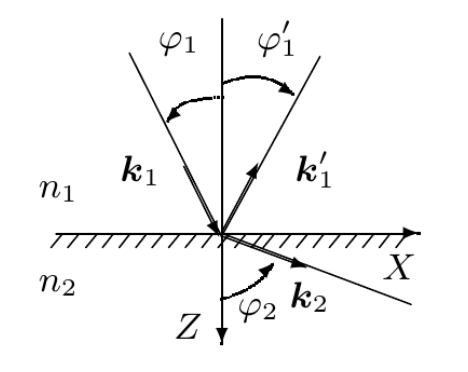
\includegraphics[width=0.3\linewidth]{img3.png}
\caption{Отражение и преломление волны на границе раздела двух сред}
\label{img3}
\end{figure}

Пусть $\vec{E_1}, \vec{E_1'}, \vec{E_2}$ - электрические поля в падающей, отраженной и преломленной волнах соответственно:
$$\vec{E_1}=\vec{a_1}e^{ik_1'(x\sin{\varphi_1}+z\sin{\varphi_1})}e^{-iw_1t}, \quad
\vec{E_1'}=\vec{a_1'}e^{ik_1'(x\sin{\varphi_1'}+z\sin{\varphi_1'})}e^{-iw_1't}, \quad
\vec{E_2}=\vec{a_2}e^{i(k_{2x}x+k_{2z}z)}e^{-iw_2t}.$$
Здесь $\varphi_1$ - угол падения, $\varphi_1'$ - угол отражения, $\varphi_2$ - угол преломления. Граничные условия с учетом этих формул:
$$
\vec{a_{1\tau}}e^{ik_1x\sin{\varphi_1}}e^{-iwt} + \vec{a'_{1\tau}}e^{ik_1'x\sin{\varphi_1'}}e^{-iw_1't} = \vec{a_{2\tau}}e^{ik_{2x}x}e^{-iw_2t}
$$
Т.к. это равенство верно при любых $x$ и $t$, то
$$
w_1 = w_1' = w_2
$$
$$
k_1\sin{\varphi_1}=k_1'\sin{\varphi_1'}=k_{2x}
$$

Отсюда получаем, что угол падения равен углу отражения: $\sin{\varphi_1}=\sin{\varphi_1'}$ и равенство: $\frac{\sin{\varphi_2}}{\sin{\varphi_1}}=\frac{k_1}{k_2} = \frac{v_2}{v_1} = \frac{n_1}{n_2} = n$.

Критическое значения угла падения наз. \textit{предельный угол полного внутреннего отражения}: 
$$
\sin{\varphi_\text{пр}} = \frac{k_2}{k_1} = \frac{n_2}{n_1} = \frac{1}{n}
$$

Теперь предположим, что волна во второй среде неоднородна. При $\varphi_1>\varphi_\text{пр}$:
$$
k_1\sin{\varphi_1} > k_1\sin{\varphi_\text{пр}} = k_1\frac{k_2}{k_1}=k_2
$$
$$
k_{2z} = \pm\sqrt{k_2^2-k_{2x}^2} = \pm i\sqrt{k_{2x}^2-k_2^2} = \pm i\sqrt{k_1^2\sin^2{\varphi_1}-k_2^2}
$$
Величина $k_{2z}$ мнимая, значит, волна во второй среде является однородной. 
$$
\chi = \sqrt{k_1^2\sin^2{\varphi_1}-k_2^2}
$$
Таким образом, электромагнитное поле во второй среде экспоненциально затухает с удалением поверхности раздела. Это экспоненциальная функция в виде $exp(-z/2\Lambda)$, где $\Lambda=\frac{1}{2}\chi$. Тогда интенсивность волны:
$$
I \varpropto e^{-z/\Lambda}
$$
Длина затухания $\Lambda$ может быть представлена в виде:
$$
\Lambda = \frac{1}{2\sqrt{k_1^2\sin^2{\varphi_1}-k_2^2}} = \frac{1}{2k_2\sqrt{n^2\sin^2{\varphi_1}-1}} = \frac{\lambda_2}{4\pi\sqrt{n^2\sin^2{\varphi_1}-1}}
$$
Эта формула позволяет количественно исследовать затухание электромагнитных колебаний во второй среде.

Проникновение электромагнитных волн через менее плотную срежу при подном внутреннем отражении - явление той же прирожы, что и происхождение частиц через область, где их полная энергия оказывается меньше потенциальной энергии. Это явление наз. \textit{туннельный эффект}. Классическим примером туннельного эффекта является $\alpha$-распад радиоактивных ядер. По аналогии с этим эффектом прохождение электромагнитных волн через узкий зазор при углах падения, превосходящих угол полного внутреннего отражения, часто наз. \textit{туннелированием}.

\section{Экспериментальная установка}

Туннелирование миллиметровых радиоволн через тонкий воздушный зазор переменной толщины изучается на установке(рис. \ref{img4}). Источник радиоволн - высокочастотный генератор Г4-115 на трех отражательных клистронах, перекрывающих полосу частот от 25.8 Ггц до 37.5 Ггц. Клистрон возбуждает в прямоугольном металлическом волноводе электромагнитную волну, которая распространяется вдоль волновода и с помощью рупорной антенны $A_1$ излучается в пространство. Электрический вектор этой волны перпендикулярен широкой стенке волновода.

\begin{figure}[h]
\centering
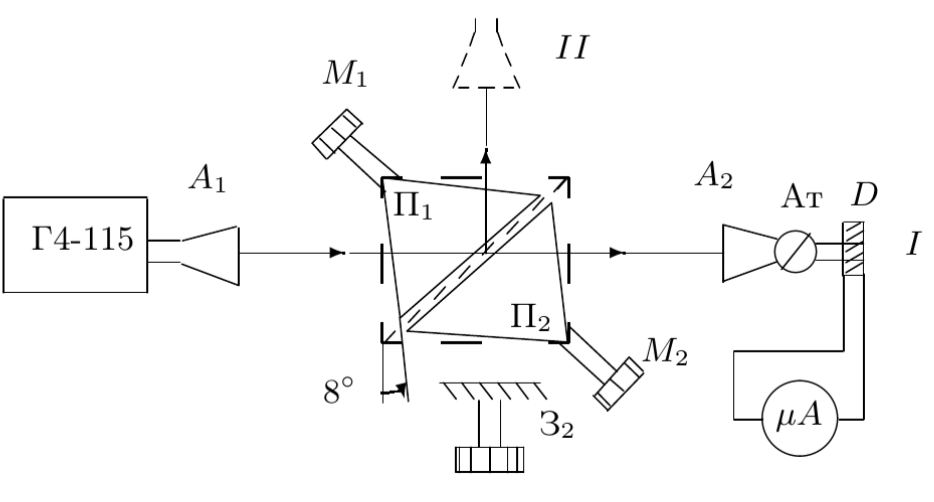
\includegraphics[width=0.7\linewidth]{img4.png}
\caption{Схема установки для исследования туннедирования миллиметровых радиоволн}
\label{img4}
\end{figure}

На пути радиоволн устанавливаются две одинаковые прямые призмы $\text{П}_1$ и $\text{П}_2$. Уменьшение угла при вершине сделано для устранения обратных отражений. Призмы изготовлены из фторопласта, обладающего малыми потерями на высоких радиочастотах. Узкие грани призм ограничивают воздушную прослойку, ширина которой может изменяться с помощью микрометрических винтоа $M_1$ и $M_2$. 

Вторая рупорная антенна $A_2$ служит приемником радиоволн. Попадая в нее, электромагнитная волна распрострарняется далее по волноводу. Детектор $D$, расположенный в волноводе, подсоедняется к микроамперметру. Аттенюатор $A_T$ позволяет ослаблять сигнал. В положении I антенна $A_2$ принимает сигнал, прошедший воздушный промежуток, в положении II - сигнал, отраженный от воздушного промежутка.

На рис.\ref{img5} представлен интерферометр Майкельсона. Воздушный зазор между призмами здесь используется в качестве делителя волны; зеркало $\text{З}_1$ установлено неподвижно, зеркало $\text{З}_2$ может перемещаться с помощью микрометрического винта $M$.

\begin{figure}[h]
\centering
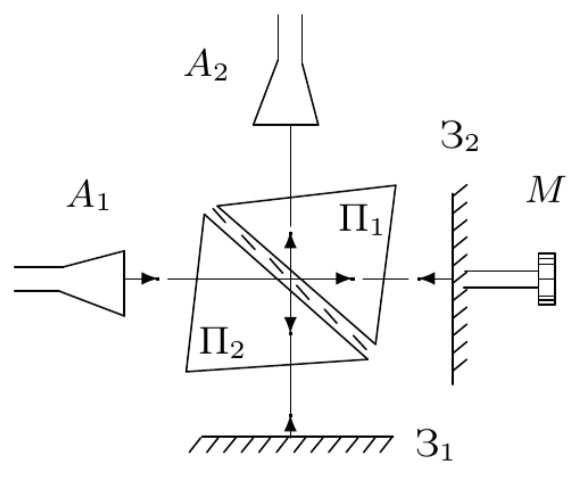
\includegraphics[width=0.4\linewidth]{img5.png}
\caption{Схема, моделирующая интерферометр Майкельсона}
\label{img5}
\end{figure}

Для измерения показателя преломления материала призм интерференционным методом перед неподвижным зеркалом устанавливается пластинна известной толщины $h$ из того же материала, что и призмы. В этом плече интерферометра возникает приращение длины "оптического" пути:
$$
\Delta = 2h(n-1)
$$
Это приращение можно скомпенсировать, передвинув подвижное зеркало на расстояние $\delta x$: $\delta x = h(n-1)$. Отсюда определяется показатель преломления.

\section{Ход работы}

\subsection{I. Подготовка приборов к работе}

\begin{enumerate}
    \item Настроим генератор по техническому описанию
    \item Установим столик с призмами так, чтобы воздушный зазор был ориентирован под углом $45^\circ$ к падающему лучу. Вращая левый и правый микрометры $M_1$ и $M_2$, убираем воздушный промежуток.
    \item Расположим приемную антенну на одной прямой с передатчиком. Снимаем металлическое зеркало, стоящее на пути луча. Слегка поворачивая столик и приемную антенну вокруг вертикальной оси, добиваемся максимального отклика микроамперметра и закрепляем оба рейтера
    \item Вращением ручек генератора настраиваем на максимальную выходную мощность клистрона. Если ток слишком велик, уменьшаем его, вращая ручку аттенюатора $A_T$.
    \item Вращением ручки 8 добиваемся загорания контрольной лампочки 10 и определим рабочую частота клистрона по шкале 9: $\nu=36\text{ГГц}$. Рассчитаем соответствующую длину волны: $\lambda=\frac{c}{\nu}=8.3\text{мм}$
\end{enumerate}

\subsection{II. Исследование туннелирования радиоволн}
\begin{enumerate}
    \setcounter{enumi}{5}
    \item Снимаем зависимость интенсивности прошедней волны от величины зазора $l$ (если с увеличением зазора интенсивность монотонно падает, значит, призмы ориентированы правильно)
    
    \begin{table}[h!]
    \centering
        \begin{tabular}{||c|c|c|c||} 
        \hline
        № & $l$, мм & I, мкА & $T=\frac{I}{I_\text{max}}$ \\ [0.5ex] 
        \hline\hline
        1 & 2.0 & 77 & 0.77 \\ 
        2 & 2.5 & 60 & 0.6 \\
        3 & 3.0 & 51 & 0.51 \\
        4 & 3.5 & 38 & 0.38 \\
        5 & 4.0 & 29 & 0.29 \\
        6 & 4.5 & 22 & 0.22 \\
        7 & 5.0 & 16 & 0.16 \\ [1ex] 
        \hline
        \end{tabular}
    \end{table}
    \item Переставляем приемний для измерения отраженного сигнала. Слегка поворачивая столики приемник, добиваемся, чтобы отклик амперметра на отраженный сигнал при максимальном зазоре был равен отклику на прощедщий сигнал при нулевом зазоре.

    Снимаем зависимость интенсивности прошедней волны от величины зазора $l$
    
    \begin{table}[h!]
    \centering
        \begin{tabular}{||c|c|c|c||} 
        \hline
        № & $l$, мм & I, мкА & $R=\frac{I}{I_\text{max}}$  \\ [0.5ex] 
        \hline\hline
        1 & 2.0 & 48 & 0.48 \\ 
        2 & 2.5 & 64 & 0.64 \\
        3 & 3.0 & 71 & 0.71 \\
        4 & 3.5 & 82 & 0.82 \\
        5 & 4.0 & 87 & 0.87 \\
        6 & 4.5 & 95 & 0.95 \\
        7 & 5.0 & 98 & 0.98 \\ [1ex] 
        \hline
        \end{tabular}
    \end{table}

    \item Для следующего пункта устанавливаем величину зазора, при которой ток равен половине максимального.
    \newpage
    \item Построим на одном листе графики зависимости коэффициентов T и R от величины зазора $l$, отнормировав токи на величину $I_{max}$

    \begin{figure}[h]
    \centering
    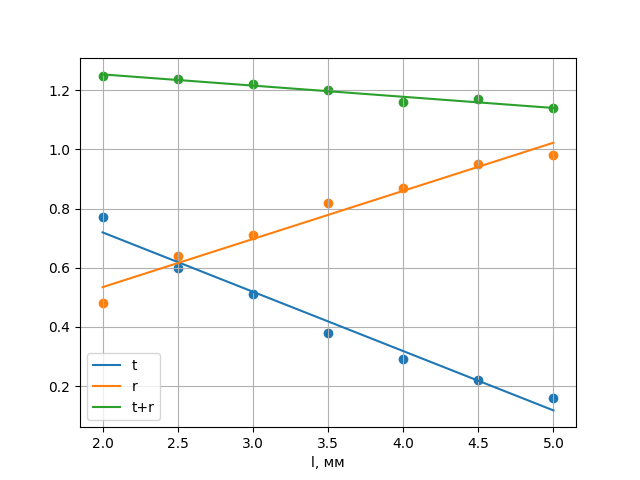
\includegraphics[width=0.65\linewidth]{graph1.png}
    \caption{Зависимость коэффициентов преломления и отражения и их суммы от величины зазора}
    \label{graph1}
    \end{figure}
    
    \item Построим график $ln(T)=f(z)$, где $z$ - показания микрометра

    \begin{figure}[h]
    \centering
    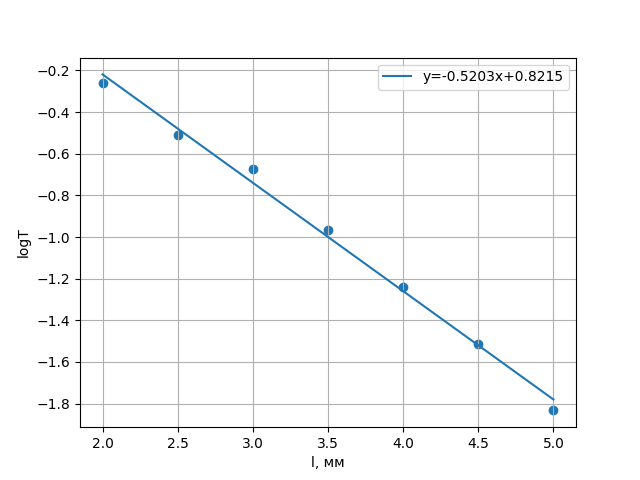
\includegraphics[width=0.65\linewidth]{graph2.png}
    \caption{Зависимость ln(T) от показаний микрометра}
    \label{graph2}
    \end{figure}
    

    По наклону прямой рассчитаем длину затухания $\Lambda$:
    $$
    \Lambda = 0.5203 \text{мм}^{-1} \pm 0.142
    $$
    
    Рассчитаем величину показателя преломления фторопласта $n$:
    $$
    n=\frac{\sqrt{16\pi\Lambda^2+\lambda_2^2}}{4\pi\Lambda\sin\varphi_1} = 1.637 \pm 0.194
    $$
    
\end{enumerate}
\newpage
\subsection{III. Интерферометр Майкельсона}
\begin{enumerate}
    \setcounter{enumi}{10}
    \item Собираем схему интерферометра Майкельсона, используя в качестве делителя зазор между призмами.
    \item Снимаем зависимость тока от координаты $x$ подвижного зеркала.
    
    \begin{table}[h!]
    \centering
        \begin{tabular}{||c|c|c||} 
        \hline
        № & x, мм & I, мкА \\ [0.5ex] 
        \hline\hline
        1 & 0.05 & 50 \\ 
        2 & 0.10 & 52 \\
        3 & 0.15 & 55 \\
        4 & 0.20 & 59 \\
        5 & 0.25 & 62 \\
        6 & 0.30 & 67 \\
        7 & 0.35 & 70 \\ [1ex] 
        \hline
        \end{tabular}
    \end{table}
    
    По графику $I = f (x)$ определим экспериментальное значение длины волны ЭМ-излучения.

    \begin{figure}[h]
    \centering
    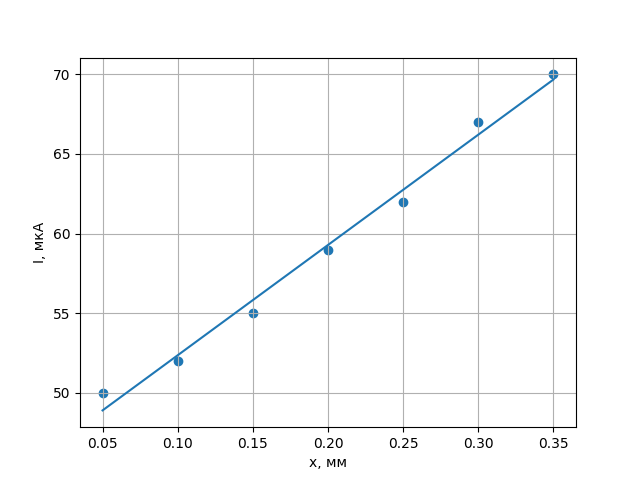
\includegraphics[width=0.65\linewidth]{graph3.png}
    \caption{Зависимость тока от координаты $x$}
    \label{graph3}
    \end{figure}
    
    \item Для измерения показателя преломления фторопласта интерфереционным методом настроим интерферометр на мксимальную интенсивность и поместим пластину известной толщины $d = 6.2\text{мм}$ перед неподвижным зеркалом. Скомпенсируем возникшее увеличение "оптической" длины пути, отодвинув от призм подвижное зеркало на необходимое расстояние $\delta x$. Рассчитаем показатель преломления фторопласта по формуле: $\delta x = h(n-1)$
    $$
    \delta x = 3.5\text{мм} \pm 0.1\text{мм}
    $$
    $$
    n = \frac{\delta x}{d} + 1 = 1.565 \pm 0.141
    $$

    \item Сравним результаты измерения преломления фторопласта $n$ интерференционным методом и методом туннелирования:
    $$
    n_\text{интерф} = 1.565 \pm 0.141
    $$
    $$
    n_\text{туннел} = 1.637 \pm 0.194
    $$
\end{enumerate}

\section{Выводы}
Мы изучили эффект проникновения электромагнитных волн(туннелирование) через воздушный зазор между диэлектрическими призмами при полном внутреннем отражении на границе диэлектрик-воздух. Также смоделировали интерферометр Майкельсона с использованием этого эффекта и измерили показатель преломления фторопласта для миллиметровых радиоволн. Значения получились близкими к табличным. Возможно, результат при измерении с помощью туннелирования получился с большей ошибкой из-за неточности в измерении тока.


\end{document}